\documentclass{beamer}
\usepackage[spanish,activeacute]{babel}
\usepackage[utf8]{inputenc}
\usepackage{listings}
\usepackage{color}

\definecolor{gray2}{rgb}{100,100,100}
\definecolor{red}{rgb}{255,0,0}
\usetheme[backgroundimagefile=img/linux]{diepen}

\author{\large Cristián Maureira Fredes\\\normalsize saint@archlinux.cl}
\title{\huge Bienvenidos a Linux}
\subtitle{\Large \textit{``Let's share the wisdom!''}}
\institute{Universidad Técnica\\ Federico Santa María}
\date{\today}

\begin{document}

\begin{frame}[t,plain]
\titlepage
\end{frame}

\section{Agenda}
\frame
{
\frametitle{Agenda}
\begin{columns}
   \begin{column}{0.5\textwidth}
	\begin{itemize}
		\item Introducción
		\item Aclaraciones
		\item Historia
		\item Características
		\begin{itemize}
			\item Entornos Graficos
			\item Distribuciones
			\item Metodología de Desarrollo
		\end{itemize}
	\end{itemize}
	\end{column}

	\begin{column}{0.5\textwidth}
	\begin{itemize}
		\item Ambientes
		\begin{itemize}
			\item Computador de Escritorio
			\item Estación de Juegos
			\item Servidor
			\item Sistemas embebidos.
		\end{itemize}
		\item Comparaciones
		\item Casos de Éxito
		\item Conclusiones
	\end{itemize}
   \end{column}
\end{columns}
}

\frame
{
\frametitle{}
\begin{center}
	\Huge{Introducción}
\end{center}
}

\frame
{
\frametitle{Introducción}
\Large{¿Qué \textbf{no} es Linux?}
\normalsize
\begin{center}
	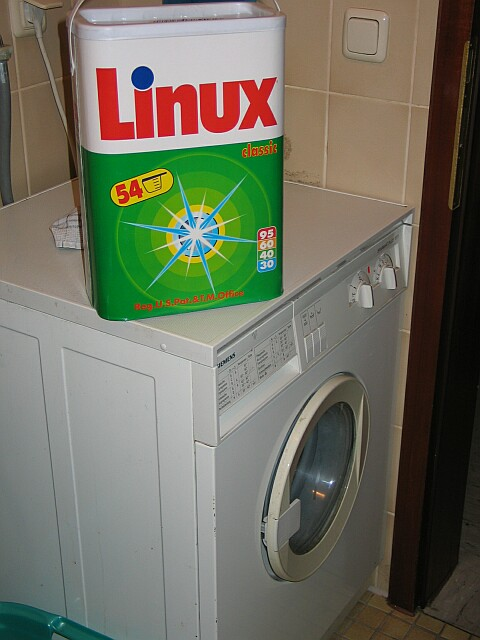
\includegraphics[width=4cm]{img/detergente-linux}
\end{center}
}

\frame
{
\frametitle{Introducción}
\Large{¿Qué \textbf{no} es Linux?}
\normalsize
15 Mitos sobre Linux
\begin{description}
	\item[1:] Si uso Linux me quedaré aislado del resto
	\item[2:] Linux no está estandarizado
	\item[3:] Sólo un experto programador puede instalar y usar Linux
	\item[4:] Linux está bien como juego, pero no para algo serio
	\item[5:] Linux no genera empleos
	\item[6:] Linux es feo
	\item[7:] En Linux no hay aplicaciones
	\item[8:] Linux es gratis y por tanto, lo que se haga en él no se puede cobrar
\end{description}
}
\frame
{
\frametitle{Introducción}
\Large{¿Qué \textbf{no} es Linux?}
\normalsize
15 Mitos sobre Linux
\begin{description}
	\item[9:] Linux es difícil de manejar
	\item[10:] En el software libre no hay innovación
	\item[11:] Todo mundo puede ver el código de los programas libres y por eso son inseguros
	\item[12:] El software libre es comunista
	\item[13:] No hay virus en Linux porque poca gente lo usa
	\item[14:] En linux no hay soporte
	\item[15:] Linux no le quita mercado a Windows, sino a Unix
\end{description}
}

\frame
{
\frametitle{Introducción}
\Large{¿Qué es Linux?}
\normalsize
\begin{itemize}
	\item Linux es un Sistema Operativo.
	\item No es el producto de una gran compañia.
	\item Es el resultado de una colaboracion entre compañias y personas.
	\item Se caracteriza por:
	\begin{itemize}
		\item Es gratis.
		\item Es libre.
		\item Es confiable.
		\item Es estable.
		\item Hay de todos los sabores.
	\end{itemize}
\end{itemize}
}

\frame
{
\frametitle{}
\begin{center}
	\Huge{Aclaraciones}
\end{center}
}

\frame
{
\frametitle{Aclaraciones}
\begin{itemize}
	\item ¿GNU/Linux o Linux?
	\begin{itemize}
		\item Linux, núcleo.
		\item GNU, aplicaciones para interactuar con el núcleo.
	\end{itemize}
	\item Algunos puristas GNU, dicen que es vital el nombre GNU/Linux.
	\item ...el resto del mundo, sólo lo llama Linux.
\end{itemize}
}

\frame
{
\frametitle{}
\begin{center}
	\Huge{Historia}
\end{center}
}

\frame
{
\frametitle{Historia}
\begin{itemize}
	\item Linux hace su \textbf{aparición} a principios de la década de los 90.
	\item Un \textbf{estudiante} de informática de la Universidad de Helsinki
		llamado \emph{Linus Torvalds}, lo comenzó como un hobby.
	\item Linus nunca pensó que tanta gente se interesara en ayudarlo
		ni tampoco en lo grande que se convertiría su proyecto.
\end{itemize}
}
\frame
{
\frametitle{Historia}
\begin{itemize}
	\item Su creación estuvo \textbf{inspirado} en MINIX, un pequeño sistema Unix
		desarrollado por Andy Tanenbaum.
	\item Las primeras \textbf{discuciones} de Linux fueron por una lista de correos
		donde Linus pedía consejos y feedback.
\end{itemize}
}

\frame
{
\frametitle{Historia}
\begin{block}{Email}
	Hello everybody out there using minix -

	I'm doing a (free) operating system (just a hobby, won't be big and
	professional like gnu) for 386(486) AT clones.$\ldots$\\\vspace{0.5cm}
	Any suggestions are welcome, but I won't promise I'll implement them $:-)$\\\vspace{0.5cm}
	$\ldots$
	PS.  Yes - it's free of any minix code, and it has a multi-threaded fs. 
	It is NOT protable (uses 386 task switching etc), and it probably never
	will support anything other than AT-harddisks, as that's all I have :-(. 
\end{block}
}

\frame
{
\frametitle{}
\begin{center}
	\Huge{Características}
\end{center}
}
% Distribuciones
\frame
{
\frametitle{Distribuciones}
\begin{center}
	
\includegraphics[width=10.5cm]{img/logos-linux}
\end{center}
}

\frame
{
\frametitle{Distribuciones}
\vspace{1cm}
\begin{center}
	
\includegraphics[width=5cm]{img/debian}
\end{center}
}

\frame
{
\frametitle{Distribuciones}
\Large{Debian}
\normalsize
\begin{itemize}
	\item El Proyecto debian es una comunidad conformada por desarrolladores y usuarios.
	\item Mantiene un sistema operativo GNU basado en software libre precompilado y empaquetado.
	\item Apuesta por separar en sus versiones el software libre del software no libre.
	\item Modelo de desarrollo ajeno a motivos empresariales o comerciales.
	\item El principal orgullo de GNU.
\end{itemize}
}

\frame
{
\frametitle{Distribuciones}
\vspace{1cm}
\begin{center}
	
\includegraphics[width=5cm]{img/redhat}
\end{center}
}

\frame
{
\frametitle{Distribuciones}
\Large{Red Hat}
\normalsize
\begin{itemize}
	\item Red Hat es la compañia responsable de la creación y mantenimiento del SO Linux \emph{Red Hat Enterprise Linux}
	\item Patrocina jboss.org y distribuye la versión profesional bajo la marca JBoss Enterprise.
	\item Uno de las principales entedidades esforzada en apoyar el movimiento del software libre.
	\item Poseen una amplia infraestructura con 2,000 empleados en 28 lugares del mundo aproximadamente.
	\item Algunas otras distribuciones basadas en Red Hat son:
	\begin{itemize}
		\item Mandriva Linux, Fedora, Yellow Dog Linux (PPC), CentOS, Scientific Linux (CERN, Fermilab LHC, ALMA)
	\end{itemize}
\end{itemize}
}

\frame
{
\frametitle{Distribuciones}
\vspace{1cm}
\begin{center}
	
\includegraphics[width=5cm]{img/ubuntu}
\end{center}
}


\frame
{
\frametitle{Distribuciones}
\Large{Ubuntu}
\normalsize
\begin{itemize}
	\item Ubuntu es una distribución Linux basda en Debian GNU/Linux.
	\item Pensada para el usuario promedio.
	\item Enfocada en la facilidad de uso.
	\item Patrocinada por Canonical Ltd. (Mark Shuttleworth)
	 \begin{itemize}
	 	\item Se financia por medio de servicios vinculados Ubuntu y soporte técnico.
	 \end{itemize}
	\item Algunas distribuciones basadas en Ubuntu son:
	\begin{itemize}
		\item Kubuntu, Xubuntu, Edubuntu y Ubuntu Server Edition
	\end{itemize}
\end{itemize}
}

\frame
{
\frametitle{Distribuciones}
\begin{center}
	
\includegraphics[width=5cm]{img/fedora}
\end{center}
}

\frame
{
\frametitle{Distribuciones}
\Large{Fedora}
\normalsize
\begin{itemize}
	\item Fedora es un SO basado en Linux, con software libre y Open Source bien actualizado.
	\item Existe una gran comunidad detrás llamada Proyecto Fedora.
	\item El Proyecto Fedora busca que sus colaboradores arreglen o contribuyan en el código del programa original, no sólo en la distribución.
	\item Es la segunda distribución más popular según DistroWatch, siendo la primera Ubuntu. 
\end{itemize}
}

\frame
{
\frametitle{Distribuciones}
\vspace{1cm}
\begin{center}
	
\includegraphics[width=6cm]{img/arch}
\end{center}
}

\frame
{
\frametitle{Distribuciones}
\Large{Arch Linux}
\normalsize
\begin{itemize}
	\item Arch Linux es una distribución GNU/Linux diseñada para ser liviana y simple.
	\item El diseño se centra en \emph{simplicidad}, \emph{elegancia}, \emph{coherencia de código} y \emph{minimalismo}.
	\item Idea central, Arch será como el usuario quiere que sea.
	\item Posee las últimas versiones de las aplicaciones y kernel.
\end{itemize}
}


% Escritorios

\frame
{
\frametitle{Entornos Gráficos}
\begin{itemize}
	\item Orientación a usuarios.
	\item Mucho más cómodo que un ambiente sólo de texto.
	\item Conjunto de elementos como:
	\begin{itemize}
		\item Ventanas
		\item Iconos
		\item Barras de herramientas
	\end{itemize}
\end{itemize}
}

\frame
{
\frametitle{Entornos Gráficos}
\Large{GNOME}
\begin{columns}
	\begin{column}{0.2\textwidth}
		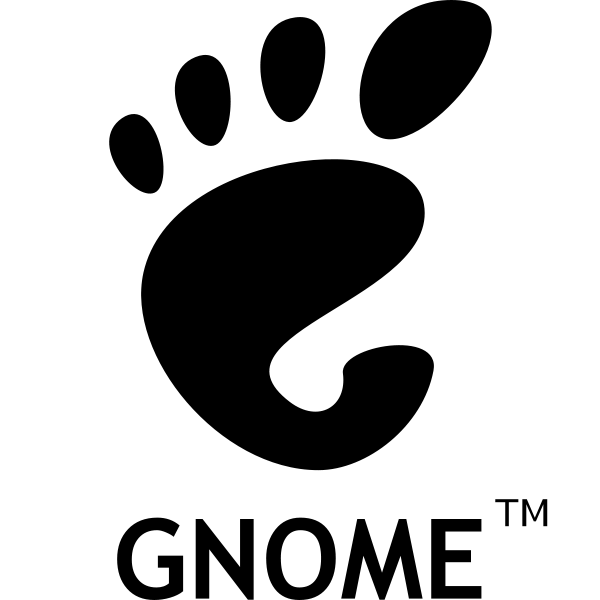
\includegraphics[width=3cm]{img/gnome-logo}
	\end{column}
	\begin{column}{0.8\textwidth}
		\begin{center}
			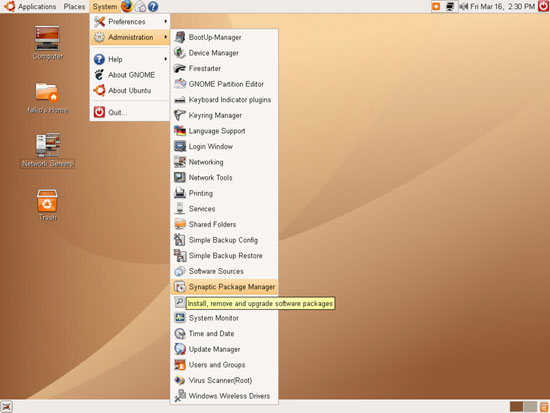
\includegraphics[width=8cm]{img/gnome}
		\end{center}
	\end{column}
\end{columns}
}

\frame
{
\frametitle{Entornos Gráficos}
\Large{KDE}
\begin{columns}
	\begin{column}{0.2\textwidth}
		
\includegraphics[width=3cm]{img/kde-logo}
	\end{column}
	\begin{column}{0.8\textwidth}
		\begin{center}
			
\includegraphics[width=8cm]{img/kde}
		\end{center}
	\end{column}
\end{columns}
}

\frame
{
\frametitle{Entornos Gráficos}
\Large{LXDE}
\begin{columns}
	\begin{column}{0.2\textwidth}
		
\includegraphics[width=3cm]{img/lxde-logo}
	\end{column}
	\begin{column}{0.8\textwidth}
		\begin{center}
			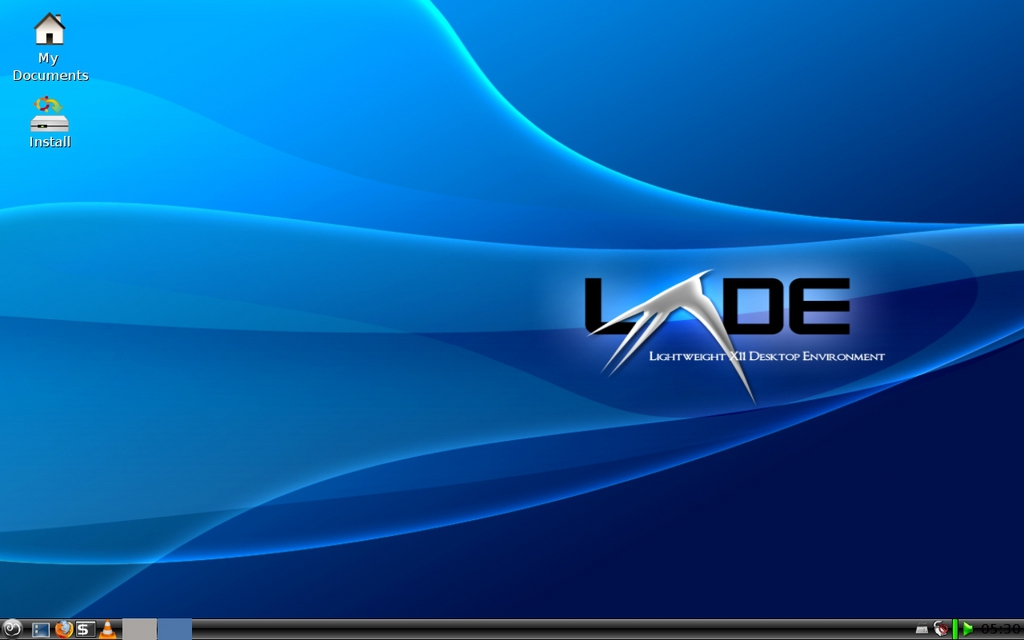
\includegraphics[width=8cm]{img/lxde}
		\end{center}
	\end{column}
\end{columns}
}

\frame
{
\frametitle{Entornos Gráficos}
\Large{XFCE}
\begin{columns}
	\begin{column}{0.2\textwidth}
		
\includegraphics[width=3cm]{img/xfce-logo}
	\end{column}
	\begin{column}{0.8\textwidth}
		\begin{center}
			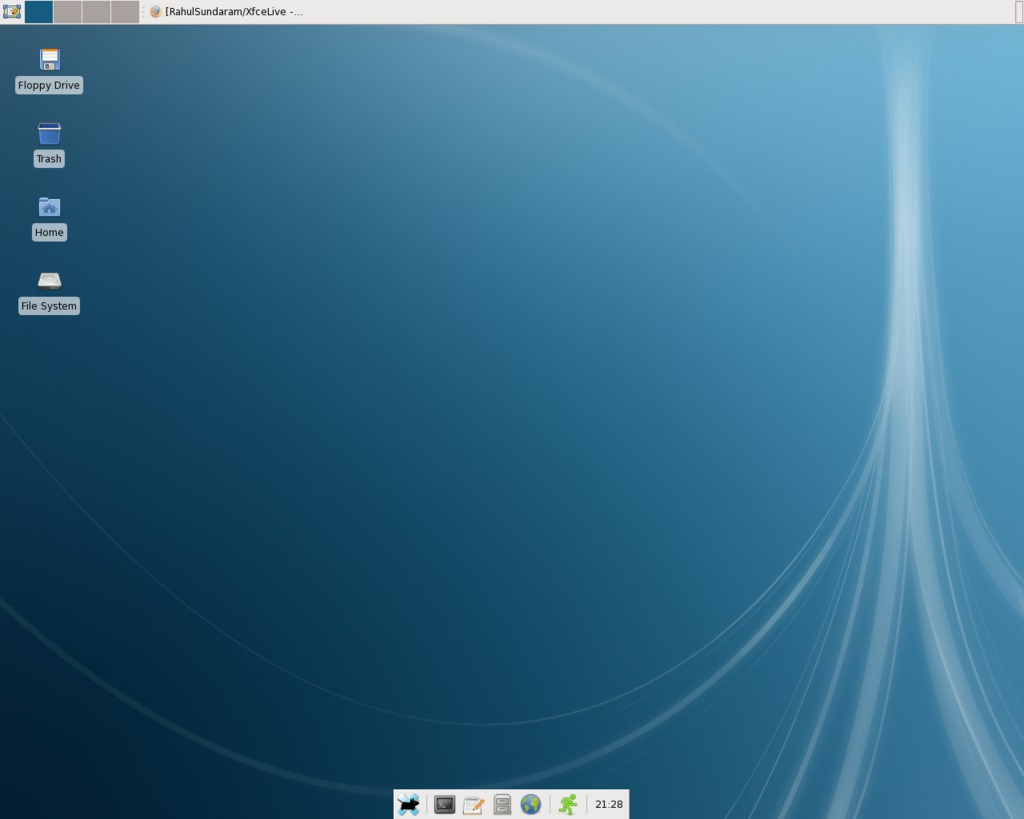
\includegraphics[width=8cm]{img/xfce}
		\end{center}
	\end{column}
\end{columns}
}

\frame
{
\frametitle{Entornos Gráficos}
\begin{itemize}
	\item Existen varios entornos gráficos aparte de los nombrados.
	\item ...y que no son malos ni nada por el estilo.
	\begin{itemize}
		\item FluxBox, BlackBox, OpenBox, Enlightenment, WindowsMaker, IceWM, FVWM, etc.
	\end{itemize}
\end{itemize}
}

\frame
{
\frametitle{Modelo de Desarrollo}
\begin{itemize}
	\item El paradigma Cliente/Usuario no se cumple del todo.
	\begin{itemize}
		\item Colaboraciones internacionales
		\item Cualquier persona puede arreglar un bug de un programa importante
	\end{itemize}
	\item Todos pueden participar.
\end{itemize}
}



\frame
{
\frametitle{}
\begin{center}
	\Huge{Ambientes}
\end{center}
}

\frame
{
\frametitle{Escritorio}
\begin{itemize}
	\item Entornos para todos los gustos.
	\item Diferentes rendimientos dependiendo del entorno.
	\item Aplicaciones necesarias disponibles
	\begin{itemize}
		\item Suite de ofimática.
		\item Navegadores.
		\item Multimedia
		\item Herramientas de desarrollo
		\item Mensajería instantánea.
	\end{itemize}
	\item Efectos visuales.
\end{itemize}
}

\frame
{
\frametitle{Estación de Juegos}
\begin{itemize}
	\item Miles de Juegos OpenSource y Libres.
	\begin{itemize}
		\item Warsow (FPS), OpenArena (Quake), Simuladores, etc.
	\end{itemize}
	\item Variados \emph{clones} de juegos populares.
	\begin{itemize}
		\item Cave Store (Castelvania), FreeCiv (Civilization II), SuperTux (SuperMario), etc.
	\end{itemize}
	\item Portings
	\begin{itemize}
		\item Doom series, Quake series, Wolfenstein, Enemy Territory
		\item Unreal Tournament 2003, 2004  y III.
	\end{itemize}
	\item Capas compatibles y Emuladores
	\begin{itemize}
		\item Wine, Cedega.
		\item Snes9x, zsnes, gnuboy, visualboy advance, VICE
	\end{itemize}
\end{itemize}
}

\frame
{
\frametitle{Servidor}
\begin{itemize}
	\item Millones de servidores en el mundo utilizan Linux.
	\begin{itemize}
		\item Google, Wikipedia, Intel, IBM, Yahoo, AMD, Nvidia, RIM, Nokia, UTFSM, etc.
	\end{itemize}
	\item Presentan niveles de seguridad, configuración y desempeño muy altos.
	\item Proveen las herramientas necesarias para montar un servidor.
	\begin{itemize}
		\item LAMP (Linux, Apache, MySQL, Perl/PHP/Python)
	\end{itemize}
	\item El $89.2\%$ de las \emph{SuperComputadoras} del mundo utilizan Linux.
	\item Linux será el SO de la computadora más poderosa del mundo, el IBM Sequoia.
	\begin{itemize}
		\item 1.6 millones de procesadores.
		\item 1.6 Petabytes de RAM.
		\item 20 petaflops (FLoating point Operations Per Second) $10^{15} flops$
		\item Un computador normal tiene un rendimiento del orden de gigaflops $10^{9} flops$
	\end{itemize}
\end{itemize}
}

\frame
{
\frametitle{Sistemas Embebidos}
\begin{itemize}
	\item Linux es el mayor competidor de Symbian OS.
	\item 16.7\% de los \emph{smarthphones} vendidos en el mundo en el 2006 tenían Linux.
	\item Actualmente variados modelos de distintas empresas corren linux
	\begin{itemize}
		\item Motorola, Nokia, Panasonic, Philips, Amazon Kindle, Google android, etc.
	\end{itemize}
	\item La mayoria de los Firewalls, routers de CISCO/Linksys usan linux.
	\item Una vez más la elección se basa en la confiabilidad y personalización de la distribución.
\end{itemize}
}

\frame
{
\frametitle{}
\begin{center}
	\Huge{Comparaciones}
\end{center}
}

\frame
{
\frametitle{Comparaciones}
\Large{¿Qué le ofrece Linux a un usuario  Windows?}
\normalsize
\begin{itemize}
	\item Adios a las restricciones.
	\item Olvidate de buscar cracks o seriales.
	\item Compartelo el software como quieras.
	\item Tienes muchas alternativas para una sola tarea.
	\item No reinicies cada vez que hay un cambio importante.
	\item Más documentación y respuestas.
	\item Portabilidad, desde un pc hasta una placa ARM.
\end{itemize}
}

\frame
{
\frametitle{Comparaciones}
\Large{¿Qué le ofrece Linux a un usuario Mac?}
\normalsize
\begin{itemize}
	\item No más programas caros.
	\item Puedes conseguir los mismos efectos visuales.
	\item Entorno más seguro.
	\item Puedes encontrar la misma facilidad de uso de Mac.
	\item Aprovechas más el rendimiento de los procesadores.
	\item Mac tiene otro enfoque...
\end{itemize}
}

\frame
{
\frametitle{}
\begin{center}
	\Huge{Casos de éxito}
\end{center}
}

\frame
{
\frametitle{Casos de éxito}
\Large{Proyectos Open Source en empresas}
\normalsize
\begin{itemize}
%Development Tools
	\item NetBeans
	\begin{itemize}
		\item IDE para desarrolladores (Soporta Java, JavaScript, C y C++)
		\item Plataformas Windows, Linux, Solaris, MacOS.
	\end{itemize}
	\item Eclipse
	\begin{itemize}
		\item IDE para desarrolladores (Soporta Java, Python, C++)
		\item Plataformas Windows, Linux, MacOS 
	\end{itemize}
	\item JUnit
	\begin{itemize}
		\item Conjunto de bibliotecas que son utilizadas en programación,
			con el objeto de hacer pruebas unitarias de aplicaciones Java.
	\end{itemize}
\end{itemize}
}
\frame
{
\frametitle{Casos de éxito}
\Large{Proyectos Open Source en empresas}
\normalsize
\begin{itemize}
	\item Valgrind
	\begin{itemize}
		\item Conjunto de herramientas de Software Libre que ayuda a depurar
			problemas de memoria y rendimiento en programas.
	\end{itemize}
	\item FindBugs
	\begin{itemize}
		\item Herramienta desarrollada por la Universidad de Maryland
				que permite el análisis estático de código, con el objeto de encontrar
				potenciales fallos por medio de búsquedas de patrones en el código.
	\end{itemize}
	\item Hibernate
	\begin{itemize}
		\item Herramienta de Mapeo objeto-relacional para Java y .Net que facilita el mapeo
			de atributos entre una Base de Datos tradicional y el modelo de objetos de una aplicación.
	\end{itemize}
\end{itemize}
}

\frame
{
\frametitle{Casos de éxito}
\Large{Proyectos Open Source en empresas}
\normalsize
\begin{itemize}
	\item SQlite
	\begin{itemize}
		\item Sistema de gestión de Bases de Datos relacional,
			contenida en una pequeña librería en C.
	\end{itemize}
	\item MySQL
	\begin{itemize}
		\item Sistema de gestión de Base de Datos relacional,
			multihilo y multiusuario con más de seis millones de instalaciones.
	\end{itemize}
	\item PostgreSQL
	\begin{itemize}
		\item Servidor de Base de Datos relacional orientado a objetos.
	\end{itemize}
\end{itemize}
}

\frame
{
\frametitle{Casos de éxito}
\Large{Proyectos Open Source en empresas}
\normalsize
\begin{itemize}
	\item Zlib
	\begin{itemize}
		\item Biblioteca de compresión de datos multiplataforma.
	\end{itemize}
	\item Libpng
	\begin{itemize}
		\item Biblioteca oficial del formato de imágenes PNG, multiplataforma
			y que contiene funciones en C para el manejo de imágenes.
	\end{itemize}
	\item FFmpeg
	\begin{itemize}
		\item Colección de Software Libre que puede grabar, convertir y hacer streaming
			de audio y video
	\end{itemize}
\end{itemize}
}

\frame
{
\frametitle{Casos de éxito}
\Large{Proyectos Open Source en empresas}
\normalsize
\begin{itemize}
	\item Pentaho Reporting
	\begin{itemize}
		\item Solución basada en el proyecto JFreeReport que permite generar informes
			de manera rápida y de gran capacidad.
	\end{itemize}
	\item JasperReports
	\begin{itemize}
		\item Herramienta para la creación de informes Java con la habilidad de entregar
			contenido rico en el monitor, en la impresora o en ficheros PDF, HTML, XLS, CSV y XML.
	\end{itemize}
	\item Prototype
	\begin{itemize}
		\item Framework escrito en JavaScript que se orienta al desarrollo de aplicaciones web,
			implementando técnicas AJAX.
	\end{itemize}
\end{itemize}
}

\frame
{
\frametitle{Casos de éxito}
\Large{Proyectos Open Source en empresas}
\normalsize
\begin{itemize}
	\item script.aculo.us
	\begin{itemize}
		\item Biblioteca JavaScript que permite el uso de controles AJAX, arrastrar y pegar,
			entre otros efectos visuales en una página web.
	\end{itemize}
	\item Direct Web Remoting
	\begin{itemize}
		\item  API de código abierto que permite realizar llamadas remotas a objetos Java del
			servidor, desde código JavaScript cliente. Utiliza la tecnología AJAX.
	\end{itemize}
	\item Yahoo! User Interface
	\begin{itemize}
		\item Son una serie de bibliotecas escritas en JavaScript para la construcción de
			 aplicaciones interactivas. Son utilizadas para la programación de aplicaciones de escritorio.
	\end{itemize}
\end{itemize}
}

\frame
{
\frametitle{Casos de éxito}
\Large{Proyectos Open Source en empresas}
\normalsize
\begin{itemize}
	\item JQuery
	\begin{itemize}
		\item Biblioteca o Framework de JavaScript que permite simplificar la manera de interactuar con documentos
			HTML, permitiendo manejar eventos, desarrollar animaciones e interactuar con AJAX.
	\end{itemize}
	\item Joomla!
	\begin{itemize}
		\item Sistema de gerencia de portales dinámicos y sistema de gestión de contenidos
	\end{itemize}
	\item Wordpress
	\begin{itemize}
		\item Sistema de gestión de contenido enfocado a la creación de blogs.
	\end{itemize}
\end{itemize}
}

\frame
{
\frametitle{Casos de éxito}
\Large{Proyectos Open Source en empresas}
\normalsize
\begin{itemize}
	\item Apache
	\begin{itemize}
		\item Servidor web HTTP de código abierto para plataformas Unix (BSD, GNU/Linux, etc.), Microsoft Windows,
			Macintosh y otras.
	\end{itemize}
	\item OpenOffice
	\begin{itemize}
		\item Suite ofimática libre que incluye herramientas como procesador de textos, hoja de cálculo,
			presentaciones, herramientas para el dibujo vectorial y base de datos.
	\end{itemize}
	\item \LaTeX
	\begin{itemize}
		\item Sistema de composición de textos, orientado especialmente a la creación de libros,
			documentos científicos y técnicos que contengan fórmulas matemáticas.
	\end{itemize}	
\end{itemize}
}

\frame
{
\frametitle{Casos de éxito}
\Large{Empresas y Organizaciones  que ocupan OpenSource}
\normalsize
\begin{itemize}
	\item Mozilla Foundation
	\begin{itemize}
		\item Firefox, Thunderbird, Bugzilla, Lightning, Sunbird, Seamonkey
	\end{itemize}
	\item SUN Microsystems (R.I.P)
	\begin{itemize}
		\item OpenOffice.org, OpenSolaris
	\end{itemize}
	\item Google
	\begin{itemize}
		\item Google Chrome, Proyectos infinitos (Google Summer of Code)
	\end{itemize}
	\item Hollywood
		\begin{itemize}
			\item Disney/Pixar, Dreamworks, Sony Pictures e Industrial Light \& Magic.
			\item \small{``Toy Story'', ``Titanic'', ``Star Wars: Episode II y III'', ``Shrek 1,2 y 3'', ``Spirit'',
				``Yo, Robot'', ``Van Helsing'', ``El señor de los anillos'', ``El Grinch'', ``Stuart Little'',
				``Harry Potter'', etc}
		\end{itemize}
	\normalsize
	\item Wikimedia
	\begin{itemize}
		\item \small{Organización matriz de Wikipedia, Wikinoticias, Wikcionario, Wikibooks, Wikiquote, Wikisource,
			Wikicommons, Wikispecies, Wikiversidad}
	\end{itemize}
\end{itemize}
}

\frame
{
\frametitle{Casos de éxito}
\Large{Empresas y Organizaciones  que ocupan OpenSource}
\normalsize
\begin{itemize}
	\item Nokia
	\begin{itemize}
		\item Sistemas Operativos de sus dispositivos más famosos, Qt.
	\end{itemize}
	\item National Radio Astronomy Observatory (NRAO)
	\begin{itemize}
		\item Servidores y Plataforma de desarrollo.
	\end{itemize}
	\item European Southern Observatory (ESO)
	\begin{itemize}
		\item Servidores y Plataforma de desarrollo
	\end{itemize}
	\item Proyecto ALMA
	\begin{itemize}
		\item El ALMA Common Software corre nativamente en Linux.
	\end{itemize}
	\item CERN
	\begin{itemize}
		\item Scientific Linux CERN 5.
	\end{itemize}
	
\end{itemize}
}
\frame
{
\frametitle{Estudios}
\Large{85\% de las empresas utilizan software Open Source}
\normalsize
\begin{itemize}
	\item Estudio realizado por la empresa consultora Gartner en el 2008.
	\item Se tomaron en cuenta datos de 274 organizaciones ubicadas en:
	\begin{itemize}
		\item America del Norte
		\item Europa
		\item Asia
	\end{itemize}
	\item El 15\% de las restante planea a corto y mediano plazo involucrarse en el mundo del Software Libre
\end{itemize}
}

\frame
{
\frametitle{Estudios}
\Large{Pero, ¿Cuáles fueron los motivos?}
\normalsize
\begin{itemize}
	\item Menores costos de manejo y capacitación del personal.
	\item No hay dependencia a un solo y monopólico proveedor de software.
	\item Rapidez de implementación al interior de la organización
	\begin{itemize}
		\item Sin sistemas o controles de validación.
	\end{itemize}
	\item Adaptabilidad del software a los requisitos de la empresa.
	\item Costos de mantenimiento y actualización considerablemente más bajo.
\end{itemize}
}

\frame
{
\frametitle{}
\begin{center}
	\Huge{Conclusiones}
\end{center}
}

\frame
{
\frametitle{Conclusiones}
\begin{itemize}
	\item Utilizar software OpenSource nos ofrece variadas ventajas
	\begin{itemize}
		\item Reducir costos, tiempo de desarrollo, dejar atras el monopolio.
	\end{itemize}
	\item Podemos
	\begin{itemize}
		\item adaptarlo a nuestros gustos.
		\item ver lo que estamos instalando.
		\item instalarlo en todas las máquinas que queramos.
		\item etc
	\end{itemize}
	\item Colaborar con proyectos de todas partes del mundo.
	\item Compartir nuestro conocimiento.
\end{itemize}
}

\frame
{
\frametitle{FLISoL}
\Large{Festival Latinoamericano de Instalación de Software Libre}
\normalsize
\begin{center}
	
\includegraphics[width=6cm]{img/flisol}
\end{center}
\begin{itemize}
	\item {\bf Lugar:} DuocUC, Centro Tecnológico de Informática (Sede Viña del Mar).
	\item {\bf Fecha:} Sábado 29 de Mayo.
	\item {\bf Hora: } 11:00hrs a 19:00hrs.
\end{itemize}
}


\frame
{
\frametitle{}
\begin{center}
	\Huge{¿Preguntas?}
\end{center}
}

\end{document}
